\documentclass[12pt,a4paper]{article}

\usepackage[utf8]{inputenc}
\usepackage[T1]{fontenc}
\usepackage{lmodern}
\usepackage{textcomp}
\usepackage{newunicodechar}
\usepackage[margin=2.5cm]{geometry}
\usepackage{amsmath,amssymb}
\usepackage{graphicx}
\usepackage{listings}
\usepackage{xcolor}
\usepackage{hyperref}
\usepackage{fancyhdr}
\usepackage{float}
\usepackage{booktabs}
\usepackage{caption}
\usepackage{tabularx}
\usepackage{array}
\usepackage{tikz}
\usetikzlibrary{trees,positioning,shapes.geometric,arrows.meta}

% Adjust header height for fancyhdr
\setlength{\headheight}{15pt}
\addtolength{\topmargin}{-3pt}

% Romanian Unicode support for standard pdflatex
\newunicodechar{Ă}{\v{A}}
\newunicodechar{ă}{\v{a}}
\newunicodechar{Â}{\^{A}}
\newunicodechar{â}{\^{a}}
\newunicodechar{Î}{\^{I}}
\newunicodechar{î}{\^{i}}
\newunicodechar{Ș}{\c{S}}
\newunicodechar{ș}{\c{s}}
\newunicodechar{Ț}{\c{T}}
\newunicodechar{ț}{\c{t}}

\hypersetup{
    colorlinks=true,
    linkcolor=blue,
    filecolor=magenta,      
    urlcolor=cyan,
    citecolor=blue
}

% Colors for code listings
\definecolor{codebg}{gray}{0.96}
\definecolor{codegreen}{rgb}{0.13,0.55,0.13}
\definecolor{codegray}{rgb}{0.5,0.5,0.5}
\definecolor{codepurple}{rgb}{0.58,0,0.82}
\definecolor{codeblue}{rgb}{0.05,0.25,0.70}

\lstset{
    backgroundcolor=\color{codebg},
    basicstyle=\ttfamily\footnotesize,
    breaklines=true,
    breakatwhitespace=true,
    frame=single,
    rulecolor=\color{gray!40},
    keepspaces=true,
    showstringspaces=false,
    upquote=true,
    columns=fullflexible,
    tabsize=2
}

\lstdefinestyle{cstyle}{
    language=C,
    commentstyle=\color{codegreen}\itshape,
    keywordstyle=\color{codeblue}\bfseries,
    stringstyle=\color{codepurple},
    numbers=left,
    numbersep=7pt,
    numberstyle=\tiny\color{codegray},
    stepnumber=1
}

\lstdefinestyle{bashstyle}{
    language=bash,
    commentstyle=\color{codegreen}\itshape,
    keywordstyle=\color{codeblue}\bfseries,
    stringstyle=\color{codepurple},
    numbers=left,
    numbersep=7pt,
    numberstyle=\tiny\color{codegray},
    stepnumber=1
}

\lstdefinestyle{consolestyle}{
    backgroundcolor=\color{codebg},
    basicstyle=\ttfamily\footnotesize,
    breaklines=true,
    frame=single,
    rulecolor=\color{gray!40},
    numbers=none
}

% Header and Footer
\pagestyle{fancy}
\fancyhf{}
\lhead{Operating Systems -- Lab 8}
\rhead{Iulian Pavlov, FAF-241}
\cfoot{\thepage}

\begin{document}

% ============================================================================
% TITLE PAGE
% ============================================================================
\begin{titlepage}
\begin{center}
    
\includegraphics[width=0.3\textwidth]{logo.png} \\[0.2cm] 
    
    \textbf{MINISTRY OF EDUCATION, CULTURE AND RESEARCH \\ OF THE REPUBLIC OF MOLDOVA} \\[0.3cm]
    
    \textbf{Technical University of Moldova \\ Faculty of Computers, Informatics and Microelectronics \\ Department of Software and Automation Engineering} \\[1.8cm]
    
    \textbf{Iulian Pavlov, FAF-241}\\[0.5cm]
    
    \Huge \textbf{Report} \\[0.5cm]
    
    \large Laboratory work nr. 8 \\[0.5cm]
    
    \textbf{\Large Processes Talking Through Pipes, in xv6} \\[0.3cm]
    \normalsize Course: Operating Systems (Track B: build your own small OS (xv6)) \\[2.2cm]

    \begin{flushright}
        \textit{Checked by:} \\
        \textbf{Reițman Patricia}, \textit{University Assistant} \\
        Department of Software and Automation Engineering, \\
        FCIM Faculty, UTM 
    \end{flushright}
    \vfill
    
    Chișinău -- 2026
\end{center}
\end{titlepage}

\pagenumbering{roman}
\newpage
\tableofcontents
\newpage
\pagenumbering{arabic}

% ============================================================================
% 1. THEORETICAL BACKGROUND & OBJECTIVES
% ============================================================================
\section{Theoretical Background and Objectives}

\subsection{Laboratory Objectives and Scope}
Inside xv6 there is no glibc, no \texttt{strace}, and no manual pages: only the 22 system calls provided by the kernel compiled from source. The objective of Laboratory Work Nr.~8 is to utilize fundamental process and pipe primitives from the lecture to build concurrent UNIX user-space programs:
\begin{itemize}
    \item \textbf{Process and Pipe System Calls}: Directly invoking the core xv6 system calls declared in \texttt{user/user.h}:
    \begin{center}
    \small\texttt{fork()}, \texttt{exit()}, \texttt{wait()}, \texttt{pipe()}, \texttt{read()}, \texttt{write()}, \texttt{close()}, \texttt{getpid()}, \texttt{printf()}
    \end{center}
    \item \textbf{Bidirectional IPC Coordination (\texttt{pingpong})}: Exchanging a byte back and forth between parent and child processes using two distinct anonymous pipes without race conditions or self-reading.
    \item \textbf{Concurrent Prime Sieve (\texttt{primes})}: Implementing Doug McIlroy's concurrent prime sieve pipeline, chaining dynamically created filter stages connected by anonymous pipes.
    \item \textbf{Systems Programming Traps}:
    \begin{enumerate}
        \item \textit{File descriptor exhaustion}: Adhering to per-process descriptor limits (\texttt{NOFILE = 16} in \texttt{kernel/param.h}) and system-wide file table limits (\texttt{NFILE = 100}) by immediately closing unused and inherited pipe ends.
        \item \textit{Infinite pipe hanging}: Ensuring that all open write descriptors are properly closed once data transmission finishes so downstream filters observe \texttt{read() == 0} (EOF).
        \item \textit{Compiler recursion checks}: Satisfying xv6's strict build flags (\texttt{-Werror}) by declaring recursive stages with \texttt{\_\_attribute\_\_((noreturn))}.
    \end{enumerate}
    \item \textbf{Argument Passing (\texttt{xargs} -- Stretch Goal)}: Building \texttt{user/xargs.c} to consume newline-separated inputs and execute target programs with composite argument vectors using \texttt{fork()}, \texttt{exec()}, and \texttt{wait()}.
\end{itemize}

\subsection{Internal xv6 Pipe Architecture}
In xv6 (\texttt{kernel/pipe.c}), an anonymous pipe is implemented as a bounded in-memory FIFO ring buffer:
\begin{lstlisting}[style=cstyle]
struct pipe {
  struct spinlock lock;
  char data[PIPESIZE]; // 512 bytes
  uint nread;          // number of bytes read
  uint nwrite;         // number of bytes written
  int readopen;        // read fd is still open
  int writeopen;       // write fd is still open
};
\end{lstlisting}

\begin{itemize}
    \item \textbf{Synchronization}: When \texttt{read()} finds the buffer empty (\texttt{nread == nwrite}) and the write end remains open (\texttt{writeopen != 0}), the kernel calls \texttt{sleep(\&pi->nread, \&pi->lock)} to suspend the reader. When a writer issues \texttt{write()}, it appends data and calls \texttt{wakeup(\&pi->nread)}, moving sleeping readers to the \texttt{RUNNABLE} state.
    \item \textbf{EOF Generation}: When a process calls \texttt{close()} on the write end of a pipe, \texttt{pipeclose()} sets \texttt{writeopen = 0} and wakes any sleeping readers. If the buffer is empty and \texttt{writeopen == 0}, \texttt{piperead()} immediately returns \texttt{0}, signaling End-Of-File.
\end{itemize}

\newpage

% ============================================================================
% 2. PART 1: PING-PONG COMMUNICATION
% ============================================================================
\section{Part 1: Ping-Pong Communication (\texttt{pingpong.c})}

\subsection{Implementation Details}
We implemented \texttt{user/pingpong.c}. The parent sends a byte to the child through pipe \texttt{p2c}. The child reads it, prints its own PID, sends the byte back through pipe \texttt{c2p}, and terminates. The parent reads from \texttt{c2p}, prints its own PID, and reaps the child:

\begin{lstlisting}[style=cstyle]
#include "kernel/types.h"
#include "user/user.h"

int
main(int argc, char *argv[])
{
  int p2c[2], c2p[2];
  char b = 'x';

  if(pipe(p2c) < 0 || pipe(c2p) < 0){
    fprintf(2, "pingpong: pipe failed\n");
    exit(1);
  }
  if(fork() == 0){
    close(p2c[1]); /* child does not write to p2c */
    close(c2p[0]); /* child does not read from c2p */
    if(read(p2c[0], &b, 1) != 1)
      exit(1);
    printf("%d: received ping\n", getpid());
    write(c2p[1], &b, 1);
    close(p2c[0]);
    close(c2p[1]);
    exit(0);
  }
  close(p2c[0]); /* parent does not read from p2c */
  close(c2p[1]); /* parent does not write to c2p */
  write(p2c[1], &b, 1);
  read(c2p[0], &b, 1);
  printf("%d: received pong\n", getpid());
  close(p2c[1]);
  close(c2p[0]);
  wait(0);
  exit(0);
}
\end{lstlisting}

\subsection{Build and Execution Trace}
We registered \texttt{\$U/\_pingpong\textbackslash} in the \texttt{Makefile} and booted xv6 under QEMU:

\begin{lstlisting}[style=consolestyle]
$ pingpong
4: received ping
3: received pong
\end{lstlisting}

\subsection{Answers to Questions (Observe -- Part 1)}

\subsubsection*{(1) Why do you need TWO pipes, and not one shared by both directions?}
Pipes in UNIX and xv6 are strictly \textbf{unidirectional} byte streams backed by a single kernel ring buffer. If only one shared pipe were used:
\begin{itemize}
    \item When the parent writes the byte \texttt{'x'} and immediately calls \texttt{read()}, the parent would race against the child and would almost certainly read back its own byte before the child could execute.
    \item Sharing a single pipe creates data races, non-deterministic self-consumption of bytes, and deadlock conditions.
\end{itemize}
Two independent pipes (\texttt{p2c} for parent-to-child and \texttt{c2p} for child-to-parent) provide isolated channels with dedicated buffers, ensuring deterministic sequencing.

\subsubsection*{(2) Nothing in your code says "wait until the child has replied". What makes the parent wait?}
The parent is suspended by the blocking behavior of the \textbf{\texttt{read()}} system call. When the parent calls:
\begin{center}
\texttt{read(c2p[0], \&b, 1);}
\end{center}
the child has not yet written into \texttt{c2p[1]}. In \texttt{kernel/pipe.c}, because the buffer is empty and \texttt{writeopen} is non-zero, the kernel puts the parent to sleep:
\begin{lstlisting}[style=cstyle]
while(pi->nread == pi->nwrite && pi->writeopen){
  if(killed(myproc())){ ... }
  sleep(&pi->nread, &pi->lock);
}
\end{lstlisting}
The parent yields the CPU until the child writes the byte, which triggers \texttt{wakeup(\&pi->nread)} and allows the parent to resume execution.

\subsubsection*{(3) Why does the child print a larger PID than the parent?}
In xv6, process identifiers (PIDs) are allocated sequentially from a global counter in \texttt{kernel/proc.c}:
\begin{lstlisting}[style=cstyle]
int
allocpid() {
  int pid;
  acquire(&pid_lock);
  pid = nextpid;
  nextpid = nextpid + 1;
  release(&pid_lock);
  return pid;
}
\end{lstlisting}
The parent process already exists (having received PID 3 when launched by \texttt{sh}). When the parent subsequently executes \texttt{fork()}, the kernel allocates the next integer in sequence (PID 4) to the child. Therefore, the child always has a strictly higher PID than its parent.

\newpage

% ============================================================================
% 3. PART 2: CONCURRENT PRIME SIEVE
% ============================================================================
\section{Part 2: Concurrent Prime Sieve (\texttt{primes.c})}

\subsection{Design and Algorithm Architecture}
Doug McIlroy's concurrent prime sieve pipeline decomposes prime number discovery into streaming pipeline stages:
\begin{enumerate}
    \item \textbf{Generator Process}: Feeds candidate integers $2, 3, \dots, 35$ into an initial pipe.
    \item \textbf{Stage Processes}: Each stage reads its first integer $p$. Because all multiples of smaller primes have been filtered by earlier stages, $p$ is guaranteed to be prime. The stage prints \texttt{"prime p"}.
    \item \textbf{Filtering and Forwarding}: The stage forks a child stage and passes through only those subsequent numbers $n$ that satisfy $n \pmod p \neq 0$. Multiples of $p$ are dropped.
    \item \textbf{Cascade Termination}: When the input pipe reaches EOF (\texttt{read() == 0}), the stage closes its outgoing pipe, waits for its child to exit, and terminates cleanly.
\end{enumerate}

\subsection{Implementation of \texttt{user/primes.c}}
The function \texttt{stage()} is annotated with \texttt{\_\_attribute\_\_((noreturn))} to satisfy \texttt{-Werror=infinite-recursion}:

\begin{lstlisting}[style=cstyle]
#include "kernel/types.h"
#include "user/user.h"

#define LIMIT 35

void stage(int) __attribute__((noreturn));

void
stage(int in)
{
  int p, n, fd[2], pid;

  if(read(in, &p, sizeof(p)) != sizeof(p)){
    close(in);
    exit(0);
  }
  printf("prime %d\n", p);

  if(pipe(fd) < 0){
    printf("primes: pipe failed after prime %d\n", p);
    close(in);
    exit(1);
  }
  pid = fork();
  if(pid < 0){
    printf("primes: fork failed after prime %d\n", p);
    close(fd[0]); close(fd[1]); close(in);
    exit(1);
  }
  if(pid == 0){
    close(fd[1]); /* Child reads from fd[0] */
    close(in);    /* Child does not need parent's input pipe */
    stage(fd[0]);
  }
  close(fd[0]);   /* Parent writes to fd[1] */
  while(read(in, &n, sizeof(n)) == sizeof(n)){
    if(n % p != 0)
      write(fd[1], &n, sizeof(n));
  }
  close(in);
  close(fd[1]);   /* Closes write end to deliver EOF to next stage */
  wait(0);
  exit(0);
}

int
main(int argc, char *argv[])
{
  int fd[2];

  if(pipe(fd) < 0)
    exit(1);
  if(fork() == 0){
    close(fd[1]);
    stage(fd[0]);
  }
  close(fd[0]);
  for(int i = 2; i <= LIMIT; i++)
    write(fd[1], &i, sizeof(i));
  close(fd[1]);
  wait(0);
  exit(0);
}
\end{lstlisting}

\subsection{Pipeline Architecture Diagram}

\begin{figure}[H]
\centering
\resizebox{\textwidth}{!}{%
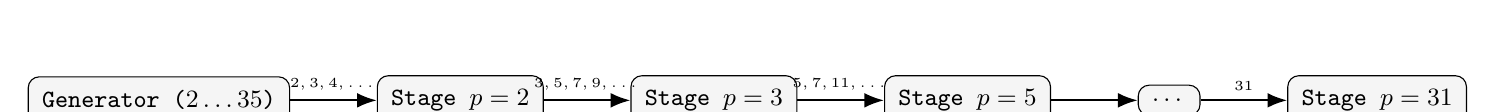
\begin{tikzpicture}[
    node distance=1.1cm,
    stage/.style={rectangle, draw, rounded corners, fill=codebg, inner sep=5pt, font=\small\ttfamily},
    arrow/.style={-{Latex[length=2.5mm]}, thick}
]
\node[stage] (gen) {Generator ($2 \dots 35$)};
\node[stage, right=of gen] (p2) {Stage $p=2$};
\node[stage, right=of p2] (p3) {Stage $p=3$};
\node[stage, right=of p3] (p5) {Stage $p=5$};
\node[stage, right=of p5] (dots) {$\dots$};
\node[stage, right=of dots] (p31) {Stage $p=31$};

\draw[arrow] (gen) -- node[above, font=\tiny] {$2,3,4,\dots$} (p2);
\draw[arrow] (p2) -- node[above, font=\tiny] {$3,5,7,9,\dots$} (p3);
\draw[arrow] (p3) -- node[above, font=\tiny] {$5,7,11,\dots$} (p5);
\draw[arrow] (p5) -- (dots);
\draw[arrow] (dots) -- node[above, font=\tiny] {$31$} (p31);
\end{tikzpicture}%
}
\caption{Streaming pipeline of concurrent filter processes connected by anonymous pipes.}
\label{fig:primesieve}
\end{figure}

\subsection{Execution Trace}
\begin{lstlisting}[style=consolestyle]
$ primes
prime 2
prime 3
prime 5
prime 7
prime 11
prime 13
prime 17
prime 19
prime 23
prime 29
prime 31
\end{lstlisting}

\subsection{Answers to Questions (Observe -- Part 2)}

\subsubsection*{(1) How many processes exist at the moment "prime 31" is printed?}
At the moment \texttt{"prime 31"} is printed, there are \textbf{12 processes} simultaneously alive in xv6:
\begin{enumerate}
    \item The original \textbf{main generator process}, which generated the input sequence $2 \dots 35$ and is currently waiting in \texttt{wait(0)} for its child to exit.
    \item Plus \textbf{11 filter stage processes}, each managing one discovered prime:
    \begin{center}
    $p \in \{2, 3, 5, 7, 11, 13, 17, 19, 23, 29, 31\}$
    \end{center}
\end{enumerate}
Because each stage stays alive while candidate numbers flow through the pipeline, all 11 stages and the main generator exist concurrently:
\begin{equation*}
    1\text{ (generator)} + 11\text{ (prime filter stages)} = \mathbf{12\text{ processes}}.
\end{equation*}

\subsubsection*{(2) Change the limit from 35 to 280. Does it still work? If not, which limit did you hit (NOFILE per process, NPROC processes, or NFILE open files in the whole system) and how did you find out?}
\begin{itemize}
    \item \textbf{Outcome}: It does not work up to 280. It correctly prints 49 primes up to \textbf{227}, and then fails on the next allocation with the diagnostic error:
    \begin{center}
    \texttt{primes: pipe failed after prime 227}
    \end{center}
    \item \textbf{Limit Hit}: The system-wide file table limit, \textbf{\texttt{NFILE = 100}} (declared in \texttt{kernel/param.h}).
    \item \textbf{Why \texttt{NFILE} and not \texttt{NOFILE} or \texttt{NPROC}}?
    \begin{enumerate}
        \item \textit{Per-process file descriptors (\texttt{NOFILE = 16})}: Every stage immediately closes \texttt{fd[0]} in the parent, \texttt{fd[1]} in the child, and the inherited input descriptors. Therefore, each process holds only 4 open file descriptors, well within \texttt{NOFILE = 16}.
        \item \textit{Process table limit (\texttt{NPROC = 64})}: 49 prime stages plus the generator equal 50 processes, which is below \texttt{NPROC = 64}.
        \item \textit{System-wide file table (\texttt{NFILE = 100})}: In xv6, every anonymous pipe requires \textbf{two} \texttt{struct file} instances in the kernel's global file table (\texttt{ftable} in \texttt{kernel/file.c})---one for read and one for write. Active stages and initial console descriptors consume all 100 slots ($49 \text{ pipes} \times 2 = 98\text{ file slots} + \text{console/sh descriptors}$). When stage 227 tries to allocate the 50th pipe, \texttt{filealloc()} returns null and \texttt{pipe()} returns $-1$.
    \end{enumerate}
    \item \textbf{How we found out}: By checking the return value of \texttt{pipe(fd) < 0} in \texttt{primes.c}. The diagnostic printed \texttt{primes: pipe failed after prime 227}. Tracing \texttt{sys\_pipe()} in \texttt{kernel/sysfile.c} reveals that \texttt{filealloc()} failed because all 100 \texttt{struct file} entries in \texttt{ftable} were exhausted.
\end{itemize}

\subsubsection*{(3) In two sentences: why is this a sieve that runs in parallel?}
Each prime filter stage executes as an autonomous concurrent process that streams non-multiples into its output pipe as soon as candidate integers arrive, rather than waiting for prior stages to process the entire dataset. Multiple integers at different filtering depths are evaluated simultaneously across CPU cores, achieving streaming pipeline parallelism.

\newpage

% ============================================================================
% 4. PART 3: STRETCH ASSIGNMENT -- XARGS
% ============================================================================
\section{Part 3: Stretch Assignment -- Implementing \texttt{xargs} (\texttt{xargs.c})}

\subsection{Specification and Design}
The \texttt{xargs} utility reads arguments from standard input and runs the specified command once per input line, appending the parsed arguments from the line:
\begin{itemize}
    \item In xv6 there is no \texttt{\$PATH} variable; \texttt{exec()} is invoked using the exact path provided.
    \item Space-separated arguments on a line are parsed into an argument vector \texttt{args[]}.
    \item For each line, \texttt{xargs} forks a child process, executes the command with \texttt{exec()}, and waits for completion.
\end{itemize}

\subsection{Implementation of \texttt{user/xargs.c}}

\begin{lstlisting}[style=cstyle]
#include "kernel/types.h"
#include "kernel/param.h"
#include "user/user.h"

int
main(int argc, char *argv[])
{
  char buf[512], *args[MAXARG], *s;
  int n, r, k, i;
  char c;

  for(i = 1; i < argc && i < MAXARG - 1; i++)
    args[i-1] = argv[i];
  int base = i - 1;

  for(;;){
    n = 0;
    while((r = read(0, &c, 1)) == 1 && c != '\n'){
      if(n < sizeof(buf) - 1)
        buf[n++] = c;
    }
    if(r != 1 && n == 0)
      break;
    buf[n] = 0;

    k = base;
    s = buf;
    while(*s && k < MAXARG - 1){
      while(*s == ' ') *s++ = 0;
      if(*s == 0) break;
      args[k++] = s;
      while(*s && *s != ' ') s++;
    }
    args[k] = 0;

    if(fork() == 0){
      exec(args[0], args);
      fprintf(2, "xargs: exec %s failed\n", args[0]);
      exit(1);
    }
    wait(0);
    if(r != 1)
      break;
  }
  exit(0);
}
\end{lstlisting}

\subsection{Execution Trace and Verification}
We verified \texttt{xargs} inside xv6:

\begin{lstlisting}[style=consolestyle]
$ echo hello too | xargs echo bye
bye hello too
\end{lstlisting}

The words \texttt{hello} and \texttt{too} were parsed from standard input and appended as additional arguments to \texttt{echo bye}, outputting \texttt{bye hello too}.

\newpage

% ============================================================================
% 5. CONCLUSIONS
% ============================================================================
\section{Conclusions}

Laboratory Work Nr.~8 provided deep, practical insights into low-level inter-process communication and concurrent systems programming in the xv6 kernel:

\begin{enumerate}
    \item \textbf{Unidirectional IPC Mechanics}: The \texttt{pingpong} experiment demonstrated why bidirectional message exchange requires two separate pipes. Synchronization is governed naturally by the kernel sleep/wakeup mechanism inside \texttt{read()} and \texttt{write()}.
    \item \textbf{Concurrent Pipeline Decomposition}: Implementing Doug McIlroy's prime sieve showcased the power of decomposing algorithmic problems into pipeline stages. Data flows concurrently through kernel ring buffers, providing pipeline parallelism across multiple processor cores.
    \item \textbf{Operating System Resource Hierarchies}: The limit 280 test demonstrated how kernel table sizing defines architectural limits. While per-process descriptor limits (\texttt{NOFILE}) and process limits (\texttt{NPROC}) were satisfied, execution halted due to the global open file table limit (\texttt{NFILE = 100}).
    \item \textbf{UNIX Pipeline Composability}: Building \texttt{xargs} completed the bridge between stream-oriented pipe outputs and argument-based program invocation, using standard \texttt{fork()}, \texttt{exec()}, and \texttt{wait()} semantics.
\end{enumerate}

\end{document}
